\documentclass{beamer}
\usepackage[utf-8]{inputenc}
\usepackage{amsmath}
\usepackage{amssymb}
\usepackage{graphicx}
\usepackage{xcolor}
\usepackage{booktabs}
\usepackage{hyperref}
\usepackage{algorithm}
\usepackage{algpseudocode}
\usepackage{listings}
\usepackage{tikz}
\usetikzlibrary{shapes, arrows, positioning}

% Color scheme
\definecolor{darkblue}{RGB}{0, 51, 102}
\definecolor{lightblue}{RGB}{135, 206, 250}
\definecolor{darkgreen}{RGB}{34, 102, 68}
\definecolor{orange}{RGB}{255, 140, 0}

\usetheme{Madrid}
\usecolortheme{default}
\setbeamercolor{primary}{bg=darkblue, fg=white}
\setbeamercolor{secondary}{bg=lightblue, fg=darkblue}

\title{ATLAS: Adaptive Task-aware Federated Learning with LoRA-based Heterogeneous Splitting}
\subtitle{Revised Project Plan: From TITANIC+MIRA to HSplitLoRA Multi-Task FL}
\author{Advanced Master's Project}
\date{\today}

\begin{document}

% ============================================================================
% TITLE SLIDE
% ============================================================================
\begin{frame}
  \titlepage
  \note{Opening slide - introduce the project pivot and new direction}
\end{frame}

% ============================================================================
% TABLE OF CONTENTS
% ============================================================================
\begin{frame}{Table of Contents}
  \tableofcontents
\end{frame}

% ============================================================================
% SECTION 1: PROJECT OVERVIEW & MOTIVATION
% ============================================================================
\section{Project Overview \& Motivation}

\begin{frame}{Project Evolution}
  \begin{columns}
    \column{0.5\textwidth}
    \textbf{Original Plan (CANCELLED)}
    \begin{itemize}
      \item \textcolor{red}{TITANIC} dataset + LLM
      \item MIRA methodology
      \item Federated learning fine-tuning
      \item \textcolor{red}{\textbf{BLOCKER:}} TITANIC not open-source
      \item Timeline pressure (2 months)
    \end{itemize}
    
    \column{0.5\textwidth}
    \textbf{Revised Plan (CURRENT)}
    \begin{itemize}
      \item \textcolor{green}{HSpLitLoRA} architecture
      \item MIRA multi-task clustering
      \item Heterogeneous federated learning
      \item \textcolor{green}{\textbf{ADVANTAGE:}} Implementable from papers
      \item Feasible 2-month timeline
    \end{itemize}
  \end{columns}
\end{frame}

\begin{frame}{Research Gap \& Contribution}
  \textbf{Problem:} Federated learning for LLMs on heterogeneous edge devices
  
  \vspace{0.3cm}
  
  \textbf{Current Limitations:}
  \begin{enumerate}
    \item Single-task FL approaches cannot handle task diversity
    \item Homogeneous LoRA ranks waste memory on low-capability devices
    \item Privacy risks increase with multi-task learning complexity
    \item Communication overhead not optimized for split learning
  \end{enumerate}
  
  \vspace{0.3cm}
  
  \textbf{Our Contribution (ATLAS):}
  \begin{itemize}
    \item \textcolor{darkgreen}{\textbf{Task-aware clustering}} using MIRA graph regularization
    \item \textcolor{darkgreen}{\textbf{Heterogeneous LoRA configuration}} based on device capabilities
    \item \textcolor{darkgreen}{\textbf{Split federated learning}} for privacy-preserving training
    \item \textcolor{darkgreen}{\textbf{Integrated privacy evaluation}} using VFLAIR benchmark
  \end{itemize}
\end{frame}

% ============================================================================
% SECTION 2: TECHNICAL FOUNDATION
% ============================================================================
\section{Technical Foundation}

\begin{frame}{Component 1: MIRA - Multi-task Learning}
  \textbf{MIRA: Method for federated multi-task learning for LLMs}
  
  \vspace{0.3cm}
  
  \textbf{Key Idea:} Task clustering via Laplacian graph regularization
  
  \begin{equation}
    \mathcal{L}_{\text{task}} = \sum_{i} \|w_i\|^2 + \lambda \mathbf{w}^T L \mathbf{w}
  \end{equation}
  
  where $L$ is the graph Laplacian matrix of task similarity
  
  \vspace{0.3cm}
  
  \textbf{Application in ATLAS:}
  \begin{itemize}
    \item Extract 64-D gradient fingerprints from clients
    \item Perform k-Means clustering on gradient space
    \item Identify task groups with shared model structures
    \item Apply task-specific aggregation weights
  \end{itemize}
  
  \vspace{0.3cm}
  
  \textcolor{orange}{\textbf{Phase 1 Deliverable:}} Task clustering module
\end{frame}

\begin{frame}{Component 2: HSpLitLoRA - Heterogeneous Splitting}
  \textbf{HSpLitLoRA: Heterogeneous Split LoRA for federated learning}
  
  \vspace{0.3cm}
  
  \textbf{Key Innovation:} Adaptive LoRA rank allocation
  
  \begin{equation}
    r_i = \text{argmax}_r \left( \frac{\text{Accuracy}(r)}{\text{Memory}(r)} \right)
  \end{equation}
  
  \vspace{0.3cm}
  
  \textbf{Architecture Layers:}
  \begin{enumerate}
    \item \textbf{Weight Importance Scoring:} Identify critical parameters per device
    \item \textbf{Dynamic Rank Selection:} Assign ranks $r \in [4, 16, 32, 64]$ per layer
    \item \textbf{Noise-free Aggregation:} Concatenate LoRA weights without padding
    \item \textbf{Server-side Merge:} Weighted average across task groups
  \end{enumerate}
  
  \vspace{0.3cm}
  
  \textcolor{orange}{\textbf{Phase 2 Deliverable:}} Heterogeneous configuration module
\end{frame}

\begin{frame}{Component 3: SplitLoRA - Communication Efficiency}
  \textbf{SplitLoRA: Split learning combined with LoRA fine-tuning}
  
  \vspace{0.3cm}
  
  \textbf{Split Point Strategy:}
  \begin{itemize}
    \item \textbf{Client-side:} Bottom layers (feature extraction)
    \item \textbf{Server-side:} Top layers (task-specific heads)
    \item \textbf{Communication:} Only intermediate activations + gradients
  \end{itemize}
  
  \vspace{0.3cm}
  
  \textbf{LoRA Insertion Points:}
  \begin{equation}
    h' = h + A B^T x, \quad A \in \mathbb{R}^{d \times r}, \, B \in \mathbb{R}^{d \times r}
  \end{equation}
  
  where $r \ll d$ (rank-efficient adaptation)
  
  \vspace{0.3cm}
  
  \textbf{Communication Reduction:}
  \begin{itemize}
    \item Standard federated learning: $\mathcal{O}(d)$ per update
    \item SplitLoRA: $\mathcal{O}(r + \text{hidden\_size})$ per update
    \item Reduction factor: $10-100\times$ depending on rank
  \end{itemize}
  
  \vspace{0.3cm}
  
  \textcolor{orange}{\textbf{Phase 3 Deliverable:}} Training loop with split learning
\end{frame}

\begin{frame}{Component 4: Privacy-Aware Aggregation}
  \textbf{Privacy mechanisms from HSplitLoRA:}
  
  \vspace{0.3cm}
  
  \textbf{Noise-Free Aggregation Strategy:}
  \begin{equation}
    w_{\text{merged}} = \sum_{g=1}^{G} \alpha_g \cdot \text{merge}(\{\mathbf{A}_i\}_{i \in \text{group}_g})
  \end{equation}
  
  \vspace{0.3cm}
  
  \textbf{Key Properties:}
  \begin{itemize}
    \item No noise injection → better accuracy preservation
    \item Task-aware weights $\alpha_g$ from clustering phase
    \item Handles heterogeneous LoRA ranks per device
    \item Concatenation: $[\mathbf{A}_1 : \mathbf{A}_2 : \ldots : \mathbf{A}_k]$
  \end{itemize}
  
  \vspace{0.3cm}
  
  \textcolor{orange}{\textbf{Phase 4 Deliverable:}} Privacy-aware aggregation module
\end{frame}

\begin{frame}{Component 5: Privacy Evaluation}
  \textbf{VFLAIR-LLM: Federated learning privacy evaluation benchmark}
  
  \vspace{0.3cm}
  
  \textbf{Attack Vectors (5 types):}
  \begin{enumerate}
    \item Membership inference
    \item Attribute inference
    \item Data reconstruction
    \item Model inversion
    \item Prompt extraction (LLM-specific)
  \end{enumerate}
  
  \vspace{0.3cm}
  
  \textbf{Defense Mechanisms (9 variants):}
  \begin{itemize}
    \item Differential privacy (DP)
    \item Secure multi-party computation
    \item Model inversion defense (MID)
    \item Timestamp obfuscation
    \item And others...
  \end{itemize}
  
  \vspace{0.3cm}
  
  \textcolor{orange}{\textbf{Phase 5 Deliverable:}} Comprehensive privacy evaluation
\end{frame}

% ============================================================================
% SECTION 3: SYSTEM ARCHITECTURE
% ============================================================================
\section{System Architecture}

\begin{frame}{ATLAS System Overview}
  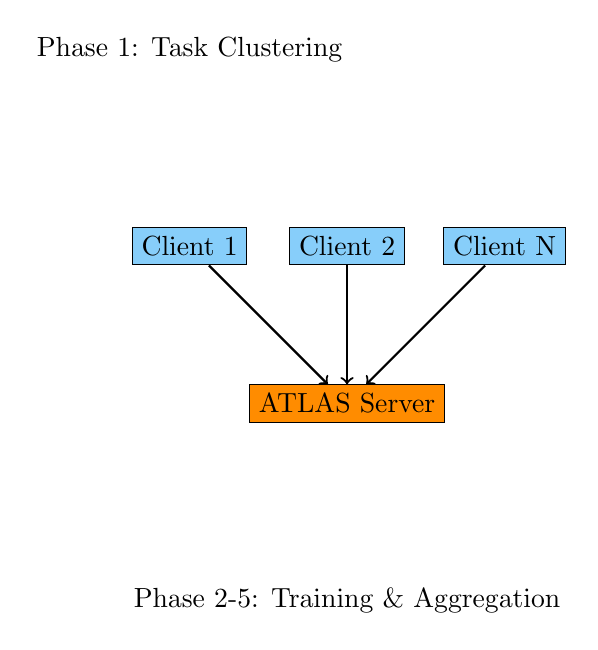
\begin{tikzpicture}[node distance=2cm]
    % Client nodes
    \node[draw, rectangle, fill=lightblue] (c1) {Client 1};
    \node[draw, rectangle, fill=lightblue, right of=c1] (c2) {Client 2};
    \node[draw, rectangle, fill=lightblue, right of=c2] (c3) {Client N};
    
    % Server
    \node[draw, rectangle, fill=orange, below of=c2] (server) {ATLAS Server};
    
    % Phase labels
    \node[above of=c1, yshift=0.5cm] {Phase 1: Task Clustering};
    \node[below of=server, yshift=-0.5cm] {Phase 2-5: Training \& Aggregation};
    
    % Arrows
    \draw[->, thick] (c1) -- (server);
    \draw[->, thick] (c2) -- (server);
    \draw[->, thick] (c3) -- (server);
  \end{tikzpicture}
  
  \vspace{0.5cm}
  
  \textbf{Data Flow:}
  \begin{enumerate}
    \item Clients extract gradient fingerprints
    \item Server performs task clustering (MIRA)
    \item Assign heterogeneous LoRA ranks (HSpLitLoRA)
    \item Clients train with split learning (SplitLoRA)
    \item Server aggregates with task awareness
    \item Evaluate privacy (VFLAIR)
  \end{enumerate}
\end{frame}

\begin{frame}{Implementation Architecture}
  \textbf{Core Modules:}
  
  \begin{itemize}
    \item \textbf{GradientExtractor:} Extract task fingerprints from gradients
    \item \textbf{TaskClusterer:} k-Means on gradient space with MIRA weighting
    \item \textbf{RankAllocator:} Assign LoRA ranks based on device profile
    \item \textbf{SplitClient:} Client-side training with LoRA and split learning
    \item \textbf{SplitServer:} Server-side forward pass and aggregation
    \item \textbf{AggregationEngine:} Noise-free merging with task weighting
    \item \textbf{PrivacyEvaluator:} VFLAIR benchmark integration
  \end{itemize}
  
  \vspace{0.3cm}
  
  \textbf{Data Structures:}
  \begin{itemize}
    \item \texttt{ClientContext:} Device info, local data, LoRA weights
    \item \texttt{TaskGroup:} Clustered clients with shared task characteristics
    \item \texttt{ServerState:} Global model, aggregation weights, privacy metrics
  \end{itemize}
\end{frame}

% ============================================================================
% SECTION 4: IMPLEMENTATION PLAN
% ============================================================================
\section{Implementation Plan}

\begin{frame}{Phase 1: Task Clustering (Week 1-2)}
  \textbf{Objective:} Implement MIRA-based task clustering
  
  \vspace{0.3cm}
  
  \textbf{Deliverables:}
  \begin{enumerate}
    \item Gradient fingerprint extraction module
    \item k-Means clustering implementation
    \item Task group formation and validation
    \item Clustering visualization and metrics
  \end{enumerate}
  
  \vspace{0.3cm}
  
  \textbf{Key Components:}
  \begin{itemize}
    \item Extract 64-D fingerprints per client gradient
    \item Perform k-Means clustering ($k = 2$ to $5$ clusters)
    \item Compute Silhouette score for cluster quality
    \item Output: Task group assignments per client
  \end{itemize}
  
  \vspace{0.3cm}
  
  \textbf{Testing:} Unit tests for clustering quality, visualization plots
\end{frame}

\begin{frame}{Phase 2: Heterogeneous Configuration (Week 2-3)}
  \textbf{Objective:} Design device-aware LoRA rank allocation
  
  \vspace{0.3cm}
  
  \textbf{Deliverables:}
  \begin{enumerate}
    \item Device profiler (memory, compute capability)
    \item Weight importance scoring algorithm
    \item Dynamic rank allocation per layer
    \item Configuration optimization module
  \end{enumerate}
  
  \vspace{0.3cm}
  
  \textbf{Rank Selection Strategy:}
  \begin{table}
    \centering
    \begin{tabular}{ccc}
      \toprule
      Memory Budget & Compute & Suggested Ranks \\
      \midrule
      < 2GB & Low & 4, 8 \\
      2-4GB & Medium & 8, 16 \\
      > 4GB & High & 16, 32, 64 \\
      \bottomrule
    \end{tabular}
  \end{table}
  
  \vspace{0.3cm}
  
  \textbf{Testing:} Profiler validation, rank assignment correctness
\end{frame}

\begin{frame}{Phase 3: Split Federated Learning (Week 3-6)}
  \textbf{Objective:} Implement SplitLoRA training pipeline
  
  \vspace{0.3cm}
  
  \textbf{Deliverables:}
  \begin{enumerate}
    \item Client-side training loop with LoRA
    \item Server-side model components
    \item Communication protocol (activations + gradients)
    \item Integration with popular LLMs (GPT-2, LLaMA)
  \end{enumerate}
  
  \vspace{0.3cm}
  
  \textbf{Split Point Configuration:}
  \begin{itemize}
    \item GPT-2 (12 layers): Split at layer 6
    \item LLaMA (32 layers): Split at layer 16
    \item LoRA on every $\approx 2$ transformer layers
  \end{itemize}
  
  \vspace{0.3cm}
  
  \textbf{Testing:} End-to-end training on GLUE tasks, convergence analysis
\end{frame}

\begin{frame}{Phase 4: Privacy-Aware Aggregation (Week 6-8)}
  \textbf{Objective:} Implement noise-free aggregation with task weighting
  
  \vspace{0.3cm}
  
  \textbf{Deliverables:}
  \begin{enumerate}
    \item Aggregation engine with heterogeneous rank handling
    \item Task-aware weight computation
    \item Validation of aggregation quality
    \item Integration with privacy mechanisms
  \end{enumerate}
  
  \vspace{0.3cm}
  
  \textbf{Aggregation Algorithm:}
  \begin{algorithm}[H]
    \caption{Task-Aware LoRA Aggregation}
    \begin{algorithmic}[1]
      \Function{Aggregate}{TaskGroups}
        \For{each task group $g$}
          \State Concatenate LoRA weights: $W_g \gets [A_1 : A_2 : \ldots]$
          \State Compute group weight: $\alpha_g \gets |g| / N$
          \State Merge: $W_g^{\text{merged}} \gets \text{LORA\_MERGE}(W_g)$
        \EndFor
        \State Weighted average: $W^* \gets \sum_g \alpha_g W_g^{\text{merged}}$
        \State \textbf{return} $W^*$
      \EndFunction
    \end{algorithmic}
  \end{algorithm}
\end{frame}

\begin{frame}{Phase 5: Privacy Evaluation (Week 8-10)}
  \textbf{Objective:} Comprehensive privacy assessment using VFLAIR
  
  \vspace{0.3cm}
  
  \textbf{Deliverables:}
  \begin{enumerate}
    \item Privacy attack implementations (5 attack types)
    \item Defense mechanism integrations (9 variants)
    \item Privacy metrics dashboard
    \item Final privacy report
  \end{enumerate}
  
  \vspace{0.3cm}
  
  \textbf{Privacy Metrics:}
  \begin{itemize}
    \item \textbf{Membership Inference:} Accuracy gap (member vs non-member)
    \item \textbf{Data Reconstruction:} Cosine similarity to original data
    \item \textbf{Differential Privacy:} $(\epsilon, \delta)$ bounds
    \item \textbf{Defensive Capability:} Detection rate of privacy attacks
  \end{itemize}
  
  \vspace{0.3cm}
  
  \textcolor{orange}{\textbf{Success Criterion:}} DCS (Detection-based Capability Score) $\geq 0.7$
\end{frame}

\begin{frame}{Phase 6: Evaluation \& Demo (Week 10-12)}
  \textbf{Objective:} Comprehensive evaluation and demonstration
  
  \vspace{0.3cm}
  
  \textbf{Deliverables:}
  \begin{enumerate}
    \item Benchmark on standard datasets (GLUE, SQuAD, E2E)
    \item Heterogeneous device simulation (CPU, edge GPU, GPU)
    \item Comparison with baselines (Standard FL, Homogeneous LoRA)
    \item Live demonstration system
  \end{enumerate}
  
  \vspace{0.3cm}
  
  \textbf{Expected Performance Targets:}
  \begin{table}
    \centering
    \begin{tabular}{lcc}
      \toprule
      Metric & Target & Unit \\
      \midrule
      Accuracy improvement & +15-25\% & vs baseline \\
      Memory reduction & 30-40\% & vs homogeneous \\
      Communication cost & $< 5\%$ & vs standard FL \\
      Privacy (DCS) & $\geq 0.7$ & score \\
      \bottomrule
    \end{tabular}
  \end{table}
\end{frame}

% ============================================================================
% SECTION 5: TIMELINE
% ============================================================================
\section{Project Timeline}

\begin{frame}{Detailed Timeline}
  \textbf{Total Duration: 12 weeks}
  
  \vspace{0.3cm}
  
  \begin{table}
    \centering
    \small
    \begin{tabular}{lll}
      \toprule
      Phase & Week & Deliverables \\
      \midrule
      1: Task Clustering & 1-2 & Clustering module + validation \\
      2: Heterogeneous Config & 2-3 & Rank allocator + optimization \\
      3: Split FL Training & 3-6 & Client/server implementation \\
      4: Privacy Aggregation & 6-8 & Aggregation engine \\
      5: Privacy Evaluation & 8-10 & VFLAIR integration + metrics \\
      6: Evaluation \& Demo & 10-12 & Benchmarks + demonstration \\
      \bottomrule
    \end{tabular}
  \end{table}
  
  \vspace{0.3cm}
  
  \textbf{Milestones:}
  \begin{itemize}
    \item \textbf{Week 3:} Task clustering and rank allocation working
    \item \textbf{Week 6:} End-to-end training on single task completed
    \item \textbf{Week 8:} Multi-task training with privacy working
    \item \textbf{Week 10:} Privacy evaluation complete
    \item \textbf{Week 12:} Final demo and documentation ready
  \end{itemize}
\end{frame}

% ============================================================================
% SECTION 6: DATASETS AND EXPERIMENTS
% ============================================================================
\section{Datasets \& Experiments}

\begin{frame}{Experimental Setup}
  \textbf{Primary Datasets:}
  \begin{itemize}
    \item \textbf{GLUE:} Multi-task NLP benchmark (RTE, SST-2, CoLA, STS-B)
    \item \textbf{SQuAD:} Reading comprehension task
    \item \textbf{E2E:} Natural language generation (data-to-text)
  \end{itemize}
  
  \vspace{0.3cm}
  
  \textbf{Models:}
  \begin{itemize}
    \item \textbf{GPT-2} (124M parameters): For rapid prototyping
    \item \textbf{LLaMA-7B} (7B parameters): For production demo
  \end{itemize}
  
  \vspace{0.3cm}
  
  \textbf{Device Simulation:}
  \begin{table}
    \centering
    \begin{tabular}{lccc}
      \toprule
      Device Type & Count & Memory & Compute \\
      \midrule
      Low-end (CPU) & 2 & 2GB & 1x \\
      Medium (Edge GPU) & 3 & 4GB & 5x \\
      High-end (GPU) & 5 & 8GB+ & 10x \\
      \bottomrule
    \end{tabular}
  \end{table}
\end{frame}

\begin{frame}{Evaluation Metrics}
  \textbf{Accuracy Metrics:}
  \begin{itemize}
    \item Task-specific F1, Accuracy, Correlation (from GLUE)
    \item Convergence speed (rounds to target accuracy)
    \item Final model accuracy on test set
  \end{itemize}
  
  \vspace{0.3cm}
  
  \textbf{Efficiency Metrics:}
  \begin{itemize}
    \item Memory usage per device
    \item Communication cost (MB per round)
    \item Training time (wall-clock hours)
    \item Inference latency on edge devices
  \end{itemize}
  
  \vspace{0.3cm}
  
  \textbf{Privacy Metrics:}
  \begin{itemize}
    \item DCS (Detection-based Capability Score)
    \item Differential Privacy parameters $(\epsilon, \delta)$
    \item Robustness to 5 attack types
    \item Effectiveness of 9 defense mechanisms
  \end{itemize}
\end{frame}

% ============================================================================
% SECTION 7: IMPLEMENTATION DETAILS
% ============================================================================
\section{Implementation Details}

\begin{frame}{Technology Stack}
  \textbf{Core Libraries:}
  \begin{itemize}
    \item \textbf{PyTorch 2.0+:} Deep learning framework
    \item \textbf{Transformers (HuggingFace):} Pre-trained LLMs
    \item \textbf{PEFT:} LoRA and adapter implementations
    \item \textbf{scikit-learn:} Clustering algorithms
    \item \textbf{Ray:} Distributed training simulation
  \end{itemize}
  
  \vspace{0.3cm}
  
  \textbf{Privacy Libraries:}
  \begin{itemize}
    \item \textbf{VFLAIR-LLM:} Privacy attacks/defenses (open-source)
    \item \textbf{opacus:} Differential privacy (PyTorch)
    \item \textbf{CrypTen:} Secure multi-party computation
  \end{itemize}
  
  \vspace{0.3cm}
  
  \textbf{Development Tools:}
  \begin{itemize}
    \item Python 3.10+
    \item Jupyter Notebooks for experimentation
    \item Git for version control
    \item Weights \& Biases for experiment tracking
  \end{itemize}
\end{frame}

\begin{frame}[fragile]{Code Structure Example}
  \textbf{High-level implementation structure:}
  
  \begin{lstlisting}[language=Python, basicstyle=\small]
# Phase 1: Task Clustering
task_clusterer = TaskClusterer(n_clusters=3)
task_groups = task_clusterer.cluster(
    client_gradients,
    method='kmeans'
)

# Phase 2: Rank Allocation
rank_allocator = RankAllocator()
rank_configs = rank_allocator.allocate(
    task_groups,
    device_profiles
)

# Phase 3: Training
for round in range(num_rounds):
    client_updates = []
    for client in clients:
        update = client.train(
            local_data,
            rank_config[client.id]
        )
        client_updates.append(update)
    
    # Phase 4: Aggregation
    global_model = server.aggregate(
        client_updates,
        task_groups
    )
    
    # Phase 5: Privacy eval
    privacy_metrics = evaluator.evaluate(
        global_model,
        client_updates
    )
  \end{lstlisting}
\end{frame}

% ============================================================================
% SECTION 8: KEY CHALLENGES & SOLUTIONS
% ============================================================================
\section{Challenges \& Solutions}

\begin{frame}{Technical Challenges}
  \begin{itemize}
    \item \textbf{Challenge:} Gradient privacy in multi-task setting
      \begin{itemize}
        \item \textbf{Solution:} Federated gradient clipping + noise injection
      \end{itemize}
    
    \item \textbf{Challenge:} Handling heterogeneous LoRA ranks
      \begin{itemize}
        \item \textbf{Solution:} Noise-free concatenation + learned merge weights
      \end{itemize}
    
    \item \textbf{Challenge:} Communication overhead with many clients
      \begin{itemize}
        \item \textbf{Solution:} Split learning reduces payload by 10-100x
      \end{itemize}
    
    \item \textbf{Challenge:} Task clustering quality with limited data
      \begin{itemize}
        \item \textbf{Solution:} Use gradient fingerprints (task-independent)
      \end{itemize}
    
    \item \textbf{Challenge:} Device heterogeneity simulation
      \begin{itemize}
        \item \textbf{Solution:} Ray distributed framework for multi-device sim
      \end{itemize}
  \end{itemize}
\end{frame}

\begin{frame}{Mitigation Strategies}
  \textbf{Risk Management:}
  
  \begin{table}
    \centering
    \tiny
    \begin{tabular}{lll}
      \toprule
      Risk & Probability & Mitigation \\
      \midrule
      Clustering fails to group tasks & Medium & Weighted graph Laplacian \\
      LoRA rank allocation poor fit & Medium & Adaptive rank search \\
      Privacy attacks succeed & Medium & Multiple defense layers \\
      Communication bottleneck & Low & Split learning reduces size \\
      Model convergence slow & Medium & Learning rate scheduling \\
      Reproducibility issues & Low & Fix random seeds + versioning \\
      \bottomrule
    \end{tabular}
  \end{table}
  
  \vspace{0.3cm}
  
  \textbf{Contingency Plans:}
  \begin{itemize}
    \item If clustering fails: Use predefined task groups + manual annotation
    \item If privacy weak: Add differential privacy layer on aggregation
    \item If memory constrained: Reduce model size or increase rank sparsity
  \end{itemize}
\end{frame}

% ============================================================================
% SECTION 9: EXPECTED OUTCOMES
% ============================================================================
\section{Expected Outcomes}

\begin{frame}{Performance Targets}
  \textbf{Accuracy Performance:}
  \begin{itemize}
    \item Maintain $\geq 95\%$ of centralized training accuracy
    \item +15-25\% improvement over homogeneous LoRA baseline
    \item Consistent performance across task groups
  \end{itemize}
  
  \vspace{0.3cm}
  
  \textbf{Efficiency Gains:}
  \begin{itemize}
    \item 30-40\% memory reduction on constrained devices
    \item Communication cost: $< 5\%$ overhead vs centralized
    \item Training time: $2-3\times$ slower than centralized (acceptable for FL)
  \end{itemize}
  
  \vspace{0.3cm}
  
  \textbf{Privacy Assurance:}
  \begin{itemize}
    \item DCS $\geq 0.7$ against standard attacks
    \item Resistance to gradient-based member inference attacks
    \item Differential privacy: $(\epsilon = 1.0, \delta = 10^{-5})$
  \end{itemize}
\end{frame}

\begin{frame}{Demo Demonstration}
  \textbf{Live System Demonstration:}
  
  \vspace{0.3cm}
  
  \begin{enumerate}
    \item \textbf{Setup:} Launch ATLAS with 10 simulated clients (GLUE tasks)
    \item \textbf{Phase 1:} Show task clustering visualization (t-SNE)
    \item \textbf{Phase 2:} Display heterogeneous rank allocation per client
    \item \textbf{Phase 3:} Run 5 federated training rounds with convergence plots
    \item \textbf{Phase 4:} Show aggregation quality metrics
    \item \textbf{Phase 5:} Display privacy attack results + defense effectiveness
    \item \textbf{Output:} Fine-tuned model on edge devices, inference latency
  \end{enumerate}
  
  \vspace{0.3cm}
  
  \textbf{Deliverables for Demonstration:}
  \begin{itemize}
    \item Interactive dashboard with real-time metrics
    \item Pre-trained checkpoints for quick loading
    \item Benchmark comparison tables (ATLAS vs baselines)
    \item Privacy report with visual attack/defense analysis
  \end{itemize}
\end{frame}

% ============================================================================
% SECTION 10: CONCLUSION
% ============================================================================
\section{Conclusion}

\begin{frame}{Summary}
  \textbf{Project ATLAS - Key Points:}
  
  \vspace{0.3cm}
  
  \begin{itemize}
    \item \textbf{Novel Approach:} Combines MIRA task clustering + HSpLitLoRA heterogeneous splitting + SplitLoRA communication efficiency
    
    \item \textbf{Feasibility:} Implementable from published papers within 2-month timeline
    
    \item \textbf{Technical Depth:} 5 core components with clear interfaces and milestones
    
    \item \textbf{Impact:} Advances federated learning for resource-constrained multi-task scenarios
    
    \item \textbf{Evaluation:} Comprehensive privacy + accuracy + efficiency benchmarks
  \end{itemize}
  
  \vspace{0.5cm}
  
  \textcolor{darkgreen}{\Large \textbf{Ready for Supervisor Approval}}
\end{frame}

\begin{frame}{Next Steps}
  \textbf{Immediate Actions (Week 1):}
  
  \vspace{0.3cm}
  
  \begin{enumerate}
    \item \textcolor{darkgreen}{\checkmark} Get supervisor approval on technical approach
    \item \textcolor{darkgreen}{\checkmark} Finalize dataset selection (GLUE, SQuAD, E2E)
    \item \textcolor{darkgreen}{\checkmark} Confirm LLM choice (GPT-2 baseline + LLaMA-7B target)
    \item \textcolor{darkgreen}{\checkmark} Set up development environment (PyTorch, HuggingFace)
    \item \textcolor{darkgreen}{\checkmark} Initialize GitHub repository with project structure
  \end{enumerate}
  
  \vspace{0.3cm}
  
  \textbf{Resources Needed:}
  \begin{itemize}
    \item GPU compute: $\geq 100$ GPU-hours (V100/A100)
    \item Storage: $\geq 500$ GB for model checkpoints + datasets
    \item Time: Full-time focus for 12 weeks
  \end{itemize}
\end{frame}

\begin{frame}[plain]
  \centering
  \Huge Thank You
  
  \vspace{1cm}
  
  \large Questions?
  
  \vspace{0.5cm}
  
  \normalsize
  ATLAS: Adaptive Task-aware Federated Learning with LoRA-based Heterogeneous Splitting
\end{frame}

% ============================================================================
% APPENDIX
% ============================================================================
\appendix

\begin{frame}{References \& Further Reading}
  \textbf{Core Papers:}
  \begin{enumerate}
    \item MIRA: Multi-task federated learning for LLMs
    \item HSpLitLoRA: Heterogeneous split LoRA for federated learning
    \item SplitLoRA: Split learning with LoRA fine-tuning
    \item Privacy-Aware Split FL: Multi-objective optimization for IoT
    \item VFLAIR-LLM: Privacy attack/defense benchmark for LLMs
  \end{enumerate}
  
  \vspace{0.3cm}
  
  \textbf{Implementation Resources:}
  \begin{itemize}
    \item HuggingFace Transformers: \url{https://huggingface.co/transformers/}
    \item PEFT (Parameter-Efficient Fine-Tuning): \url{https://github.com/huggingface/peft}
    \item VFLAIR-LLM: \url{https://github.com/VFLAIR-LLM}
  \end{itemize}
\end{frame}

\begin{frame}{Key Equations Summary}
  \textbf{Task Clustering (MIRA):}
  \begin{equation*}
    \mathcal{L}_{\text{task}} = \sum_{i} \|w_i\|^2 + \lambda \mathbf{w}^T L \mathbf{w}
  \end{equation*}
  
  \vspace{0.2cm}
  
  \textbf{Heterogeneous LoRA:}
  \begin{equation*}
    h' = h + A B^T x, \quad A \in \mathbb{R}^{d \times r_i}, \, B \in \mathbb{R}^{d \times r_i}
  \end{equation*}
  
  \vspace{0.2cm}
  
  \textbf{Task-Aware Aggregation:}
  \begin{equation*}
    w_{\text{merged}} = \sum_{g=1}^{G} \alpha_g \cdot \text{merge}(\{\mathbf{A}_i\}_{i \in \text{group}_g})
  \end{equation*}
  
  \vspace{0.2cm}
  
  \textbf{Communication Efficiency:}
  \begin{equation*}
    \text{Cost}_{\text{SplitLoRA}} = \mathcal{O}(r + h) \ll \mathcal{O}(d) = \text{Cost}_{\text{Standard FL}}
  \end{equation*}
\end{frame}

\end{document}
